% =================================================================
% Kapitel: Simulation
% =================================================================

\textit{Bearbeitet von Masoud Fahim}\\

Die Aufgabenstellung sieht vor, die Reglerauslegung vor der praktischen Umsetzung zu
simulieren. Die Simulation erfüllt dabei zwei Zwecke: Sie dient zunächst der Überprüfung
der Auslegung gegen die theoretische Erwartung und liefert anschließend die
Vergleichsgrundlage, an der sich die Messungen am Prüfstand beurteilen lassen. Die
Modellbildung erfolgte in MATLAB Simulink.

% +++++++++++++++++++++++++++++++++++++++++++++++++++++++++++++++++
% Modellaufbau und Vorgehen
% +++++++++++++++++++++++++++++++++++++++++++++++++++++++++++++++++
\section{Modellaufbau und Vorgehen}
\label{sec:modellaufbau}

\subsection*{Schrittweiser Aufbau}

Das Modell wurde nicht in einem Zug erstellt, sondern in einzelnen Ausbaustufen. Jede
Stufe fügt genau einen Effekt hinzu, und für jede Stufe wurde vor dem Simulationslauf eine
Erwartung berechnet, gegen die das Ergebnis geprüft wurde.

Dieses Vorgehen ist aufwendiger als der unmittelbare Aufbau des vollständigen Modells,
hat aber einen entscheidenden Vorteil. Das Modell enthält mehrere Nichtlinearitäten --
Stellgrößenbegrenzung, Anstiegsbegrenzung, Quantisierung, Totzone -- die sich im Ergebnis
überlagern. Werden sie gemeinsam eingebaut und weicht das Ergebnis von der Erwartung ab,
lässt sich die Ursache nicht mehr einem einzelnen Block zuordnen. Wird dagegen jeweils nur
ein Effekt ergänzt, ist im Fehlerfall unmittelbar klar, welcher Block dafür verantwortlich
ist.

Ein Beispiel aus dem Aufbau verdeutlicht das: Die Anstiegsbegrenzung war zunächst auf
500~mm/s² gesetzt. Das Modell zeigte daraufhin ein deutliches Überschwingen mit
anschließendem Pendeln. Da in diesem Schritt ausschließlich die Stellgrößengrenzen
ergänzt worden waren, war die Ursache eindeutig zuzuordnen und der Wert konnte korrigiert
werden, bevor die nachfolgenden Effekte den Befund überdeckten. Die Begründung des
korrigierten Werts findet sich in Abschnitt \ref{sec:positionsregler}.

Als Referenz für die erste Stufe diente jeweils eine analytisch berechenbare Größe, etwa
die Sprungantwort eines Verzögerungsglieds erster Ordnung. Erst wenn diese im Modell
reproduziert wurde, kam der nächste Effekt hinzu.

\subsection*{Zentrale Parameterverwaltung}

Sämtliche Zahlenwerte des Modells sind in einem MATLAB-Skript \texttt{params.m}
hinterlegt, das vor jedem Simulationslauf ausgeführt wird. Die Simulink-Blöcke enthalten
keine numerischen Werte, sondern ausschließlich Variablennamen.

Diese Trennung hat sich aus zwei Gründen bewährt. Zum einen ist eine Größe, die an
mehreren Stellen im Modell auftritt -- etwa die Abtastzeit, die sowohl im Halteglied als
auch in der Anstiegsbegrenzung wirksam wird -- nur an einer Stelle zu ändern. Zum anderen
werden dieselben Werte auch von den Auswerteskripten verwendet, die Simulation und
Messung gegenüberstellen, sodass beide Seiten des Vergleichs zwangsläufig mit identischen
Parametern arbeiten.

Zusätzlich ist jeder Parameter mit einer Kennzeichnung seiner Herkunft versehen. Tabelle
\ref{tab:parameterstatus} erläutert die verwendeten Kürzel.

% ---------------------------------------------------------------
\begin{table}[htbp]
    \centering
    \caption{Kennzeichnung der Parameterherkunft in \texttt{params.m}}
    \label{tab:parameterstatus}
    \begin{tabular}{clp{8cm}}
        \hline
        Kürzel & Bedeutung & Beispiel \\
        \hline
        {[M]} & gemessen  & Federkonstante, Mikroschritteinstellung des Treibers \\
        {[B]} & berechnet & Weg je Mikroschritt, Encoderauflösung, $K_P$ \\
        {[A]} & Annahme   & Dämpfung, Totzeit, Kennlinie von \texttt{SG\_RESULT} \\
        \hline
    \end{tabular}
\end{table}
% ---------------------------------------------------------------

Die Unterscheidung ist nicht nur dokumentarischer Natur. Sie macht sichtbar, auf welchen
Annahmen eine Aussage des Modells beruht, und damit auch, wie belastbar diese Aussage
ist. Ein Modell, dessen Ergebnis von einem als [A] gekennzeichneten Parameter abhängt,
ist nur so gut wie diese Annahme. Wie sich im weiteren Verlauf zeigte, war genau das der
entscheidende Punkt bei der Bewertung des Kraftzweigs.

\subsection*{Umfang der Modelle}

Im Rahmen der Arbeit entstanden zwei Modelle. Das erste bildet den Positionsregelkreis ab
und wurde gegen Messdaten validiert. Das zweite bildete den geplanten Kraftregelkreis über
\texttt{SG\_RESULT} ab; es wurde nach der Verwerfung des Konzepts nicht weiterentwickelt,
ist aber als Beleg für die durchgeführte Auslegung dokumentiert. An seine Stelle trat eine
Erweiterung des Positionsmodells um die Federkennlinie. Die folgenden Abschnitte behandeln
die drei Modelle in dieser Reihenfolge.

% +++++++++++++++++++++++++++++++++++++++++++++++++++++++++++++++++
% Positionsregelkreis
% +++++++++++++++++++++++++++++++++++++++++++++++++++++++++++++++++
\section{Positionsregelkreis}
\label{sec:sim_position}

Das Modell des Positionsregelkreises entstand in sechs Stufen. Die Blockstruktur
entspricht dem in Abbildung \ref{fig:positionsregelkreis} gezeigten Regelkreis; Abbildung
\ref{fig:simulink_position} zeigt die Umsetzung in Simulink.

% ---------------------------------------------------------------
\begin{figure}[htbp]
    \centering
    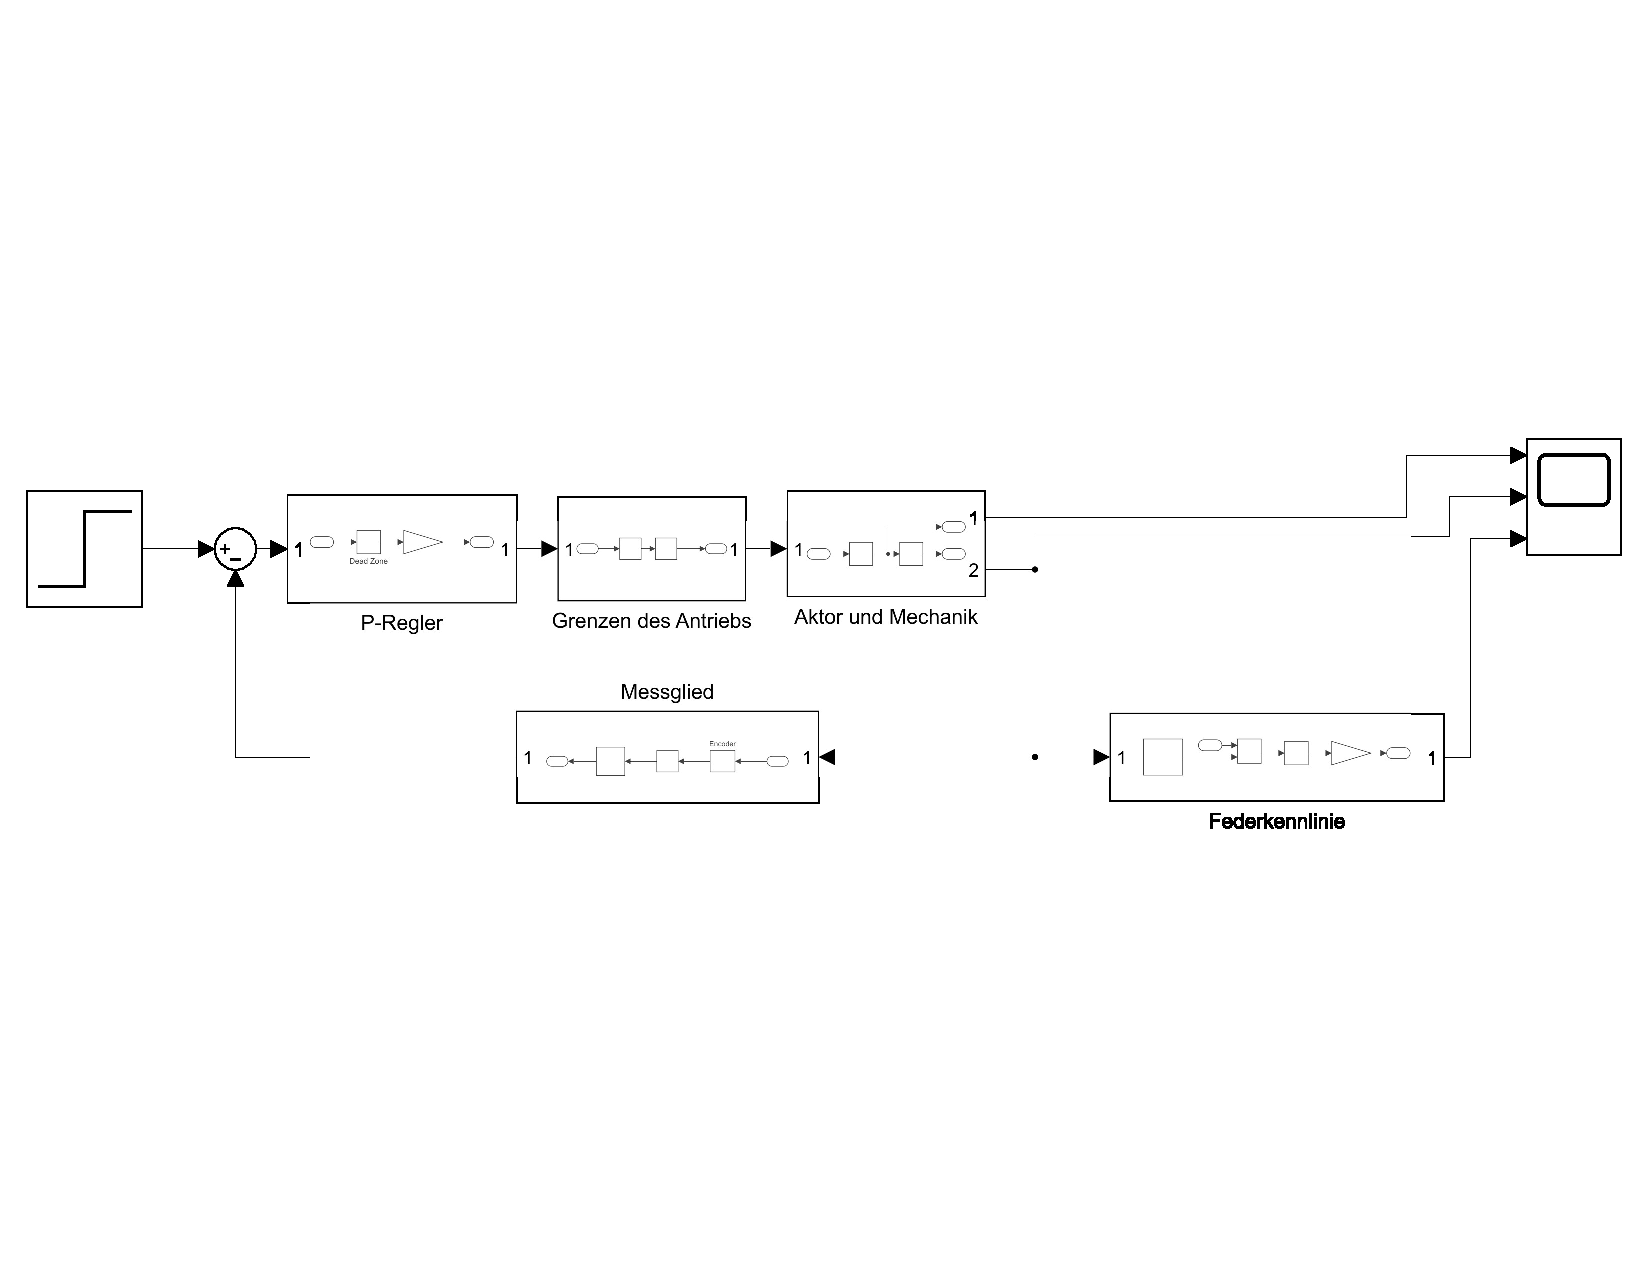
\includegraphics[width=\textwidth, trim=12pt 205pt 13pt 200pt, clip]
                    {Abbildung/Positions_Effort_Regelkreis.pdf}
    \caption{Simulink-Modell des Positionsregelkreises. Die obere Reihe bildet Regler,
             Stellgrößengrenzen sowie Aktor und Strecke ab, der linke untere Zweig das
             Messglied. Der rechte untere Zweig \texttt{Federkennlinie} berechnet die
             Kraft aus der Position und ist nicht Teil des Regelkreises
             (Abschnitt \ref{sec:sim_feder}).}
    \label{fig:simulink_position}
\end{figure}
% ---------------------------------------------------------------

\subsection*{Stufe 1: Idealmodell}

Die erste Stufe besteht aus fünf Blöcken: Sprungfunktion, Summierer, Verstärkung,
Integrator und Anzeige. Weder Abtastung noch Begrenzungen oder Quantisierung sind
enthalten. Der geschlossene Kreis entspricht damit exakt der Übertragungsfunktion

\begin{equation}
    G_w(s) = \frac{K_P}{s + K_P} ,
    \label{eq:fuehrung}
\end{equation}

also einem Verzögerungsglied erster Ordnung mit der Zeitkonstante $\tau = 1/K_P$. Als
Referenz diente der in MATLAB berechnete Verlauf von \texttt{step(tf(Kp,[1 Kp]))}.

Bei einer Sprunghöhe von 0,2~mm ergeben sich die in Tabelle \ref{tab:stufe1} genannten
Prüfpunkte. Alle drei wurden vom Modell getroffen.

% ---------------------------------------------------------------
\begin{table}[htbp]
    \centering
    \caption{Prüfpunkte des Idealmodells bei einem Sprung von 0,2~mm}
    \label{tab:stufe1}
    \begin{tabular}{llp{6cm}}
        \hline
        Zeitpunkt & Position & Bedeutung \\
        \hline
        $t = 7{,}96$~ms  & 0,1264~mm & 63,2~\%, entspricht $\tau$ \\
        $t = 23{,}9$~ms  & 0,1900~mm & 95~\%, entspricht $3\tau$ \\
        Endwert          & 0,2000~mm & keine bleibende Abweichung trotz reinem P-Anteil \\
        \hline
    \end{tabular}
\end{table}
% ---------------------------------------------------------------

Der Endwert bestätigt die in Abschnitt \ref{sec:strecke} gegebene Begründung der
P-Struktur: Obwohl der Regler keinen Integralanteil besitzt, verbleibt keine
Regelabweichung.

\subsection*{Stufe 2: Abtastung}

In der zweiten Stufe wurde ein Halteglied nullter Ordnung mit der Abtastzeit $T$ in den
Rückführzweig eingefügt. Es bildet ab, dass der Encoder nur alle 2~ms gelesen wird und
der Messwert bis zur nächsten Messung konstant bleibt. Der Kreis folgt damit der
Differenzengleichung

\begin{equation}
    x[k+1] = x[k] + K_P T \cdot \big(x_{soll} - x[k]\big) .
    \label{eq:diskret}
\end{equation}

Charakteristisch ist, dass das Verhältnis aufeinanderfolgender Geschwindigkeitsstufen
konstant bleibt und

\begin{equation}
    \frac{v[k+1]}{v[k]} = 1 - K_P T = 0{,}749
    \label{eq:polstelle}
\end{equation}

beträgt. Dieser Wert ist zugleich die Polstelle des diskreten Kreises und diente als
Prüfgröße: Im Modell ergab sich für die ersten Stufen ein Verhältnis von
$18{,}82 / 25{,}13 = 0{,}749$, in Übereinstimmung mit Gleichung \ref{eq:polstelle}.

Die Abtastung führt darüber hinaus eine Stabilitätsgrenze ein, die im kontinuierlichen
Modell der ersten Stufe nicht existiert. Bei $K_P T = 1$ erreicht der Kreis das Ziel
innerhalb eines Takts, darüber schwingt er alternierend, und ab $K_P T = 2$ läuft er auf.
Bei $T = 2$~ms entspricht das der in Tabelle \ref{tab:stabilitaetsgrenzen} genannten
Grenze von $K_P = 1000\,\mathrm{s^{-1}}$.

\subsection*{Stufe 3: Stellgrößengrenzen}

Die dritte Stufe ergänzt die Begrenzung auf $\pm v_{max}$ und die nachgeschaltete
Anstiegsbegrenzung. Die Sättigung greift, sobald die Regelabweichung den Wert

\begin{equation}
    e^{*} = \frac{v_{max}}{K_P} = \frac{40\,\mathrm{mm/s}}{125{,}7\,\mathrm{s^{-1}}}
    = 0{,}318\,\mathrm{mm}
    \label{eq:esat}
\end{equation}

überschreitet. Bei einem Sprung von 10~mm bedeutet das, dass der Antrieb über mehr als
99~\% der Fahrstrecke mit konstanter Höchstgeschwindigkeit fährt und sich das
exponentielle Verhalten des Reglers erst auf den letzten Zehntelmillimetern zeigt.

Daraus ergibt sich eine wichtige Konsequenz für die Verifikation: Zur Überprüfung von
$K_P$ sind ausschließlich Sprünge unterhalb von 0,3~mm geeignet. Bei größeren Sprüngen
misst man die Sättigungsgeschwindigkeit und erhält keinerlei Aussage über den Regler.
Beide Fälle wurden simuliert, da große Sprünge den realistischen Betriebsfall darstellen.

In dieser Stufe trat der bereits in Abschnitt \ref{sec:modellaufbau} erwähnte Fehler auf.
Die Anstiegsbegrenzung war zunächst auf 500~mm/s² gesetzt, was zu einem Überschwingen mit
anschließendem Pendeln führte. Ursache ist, dass der Regler seine Ausgangsgröße bei einem
Sprung der Höhe $\Delta x$ von sich aus mit

\begin{equation}
    \dot{v} = K_P^2 \cdot \Delta x
    \label{eq:reglerbeschleunigung}
\end{equation}

ändert, bei einem Sprung von 0,2~mm also mit rund 3160~mm/s². Eine Begrenzung unterhalb
dieses Werts bremst nicht den Antrieb, sondern den Regler. Mit 5000~mm/s² läuft der Kreis
sauber ein.

Als Nebenbefund bestätigte diese Stufe, dass trotz der langen Sättigungsphase kein Windup
auftritt. Ein PI-Regler hätte über die rund 0,24~s dauernde Sättigungsfahrt bei einem
10-mm-Sprung eine Regelabweichung von nahezu 10~mm aufintegriert und eine
Anti-Windup-Logik erfordert.

\subsection*{Stufe 4: Quantisierung}

Die vierte Stufe ergänzt zwei Quantisierer: einen im Rückführzweig für die Auflösung des
Encoders und einen vor dem Integrator für die Mikroschritte des Motors. Damit zeigt das
Modell den in Abschnitt \ref{sec:positionsregler} beschriebenen Grenzzyklus: Die
Geschwindigkeit wechselt dauerhaft zwischen kleinen positiven und negativen Werten,
anstatt auf null zu gehen.

Mit der Totzone hinter dem Summierer verschwindet dieses Verhalten, und die
Geschwindigkeit erreicht exakt null. Das Modell bestätigt damit sowohl die Ursache des
Effekts als auch die Wirksamkeit der gewählten Gegenmaßnahme.

\subsection*{Stufe 5: Totzeit}

Die fünfte Stufe ergänzt eine Totzeit im Rückführzweig, die das Lesen über I$^2$C und die
Rechenzeit im Task abbildet. Ihr Einfluss ist gegenüber der Abtastzeit von 2~ms gering;
die Phasenreserve sinkt um wenige Grad. Sichtbar wird der Effekt erst in der Nähe der
Stabilitätsgrenze und damit weit oberhalb des Entwurfswerts von $K_P$.

\subsection*{Stufe 6: Motorresonanz und Entscheidung gegen ihre Modellierung}

Die sechste Stufe sah ein Schwingungsglied zweiter Ordnung zwischen Integrator und
Abgriffpunkt vor. Es bildet ab, dass der Rotor der kommandierten Schrittfolge nicht starr
folgt, sondern als Feder-Masse-System aus magnetischer Steifigkeit und Trägheit. Diese
Stufe lieferte die in Abschnitt \ref{sec:positionsregler} diskutierte
Stabilitätsbedingung nach Gleichung \ref{eq:resonanzgrenze}.

Im finalen Modell ist dieses Glied nicht enthalten. Der Grund ist der Abgleich mit den
Messdaten: Das reine Integratormodell trifft den gemessenen Verlauf bereits im Rahmen der
Messgenauigkeit (Abschnitt \ref{sec:ergebnis_abgleich}). Eine Ergänzung des
Schwingungsglieds würde die Übereinstimmung nicht verbessern, hätte aber zwei freie
Parameter -- Eigenfrequenz und Dämpfung -- eingeführt, die beide nicht gemessen wurden.
Ein Modell mit unbestimmten Parametern, das keine bessere Übereinstimmung liefert, ist dem
einfacheren Modell nicht vorzuziehen.

Die Stabilitätsanalyse bleibt davon unberührt. Sie war als Auslegungsschritt notwendig,
um die zulässige Höhe von $K_P$ abzuschätzen, und führte zu der Entscheidung, die
Inbetriebnahme mit reduziertem Wert zu beginnen. Dass sich ihr Ergebnis im Betrieb als
unkritisch erwies, entwertet den Schritt nicht -- es begrenzt lediglich die Dämpfung des
realen Motors nach unten.

% +++++++++++++++++++++++++++++++++++++++++++++++++++++++++++++++++
% Kraftregelkreis über SG_RESULT
% +++++++++++++++++++++++++++++++++++++++++++++++++++++++++++++++++
\section{Kraftregelkreis über SG\_RESULT}
\label{sec:sim_sg}

Der in Abschnitt \ref{sec:sg_entwurf} beschriebene Kraftregelkreis wurde nach demselben
Verfahren aufgebaut wie der Positionskreis. Da die Wandlungskette zwischen Stellgröße und
Messgröße hier aus mehreren physikalischen Stufen besteht, entstand das Modell in sechs
Schritten entlang dieser Kette.

\subsection*{Aufbau entlang der Wandlungskette}

Die ersten vier Schritte bilden das Messglied ab, wobei als Eingangsgröße zunächst eine
Rampe als Platzhalter für den Antrieb diente. Erst im fünften Schritt wurde der Kreis
geschlossen.

\begin{description}
    \item[E1 -- Kontaktmodell] Federweg nach Gleichung \ref{eq:kette_weg} mit Begrenzung
          auf nichtnegative Werte, anschließend Multiplikation mit der Steifigkeit.
          Prüfpunkt: Vor dem Kontaktpunkt muss die Kraft exakt null sein und nicht
          negativ; bei doppeltem Federweg muss sich die Kraft verdoppeln.
    \item[E2 -- Momentbildung] Umrechnung der Kraft in ein Motormoment nach Gleichung
          \ref{eq:kette_moment}, anschließend Addition des Reibmoments. Prüfpunkt: vor
          dem Kontakt 15~Nmm, bei Sollkraft 100~Nmm. Dieser Schritt diente zugleich der
          Kontrolle des Faktors zwei -- eine Rechnung mit nur einer Zahnstange hätte
          57,5~Nmm ergeben.
    \item[E3 -- Kennlinie des Sensors] Fallende Gerade nach Gleichung \ref{eq:kette_sg},
          begrenzt auf den Registerbereich und quantisiert auf gerade Werte, da das
          niederwertigste Bit von \texttt{SG\_RESULT} fest null ist. Rechnerisch ergibt
          sich für die Sollkraft ein Wert von 285; im Modell erscheint 284, weil ein
          ungerader Zielwert im Register nicht existiert.
    \item[E4 -- Abtastung je Vollschritt] Quantisierung der Position auf das
          Vollschrittraster von 0,267~mm vor dem Kontaktblock. Damit springen Kraft,
          Moment und Messwert gemeinsam nur an den Vollschrittpositionen.
    \item[E5 -- Regler] Ergänzung von Fehlerbildung, Verstärkung, Begrenzungen und
          Integrator. Damit entfällt die Rampe, die Geschwindigkeit stammt nun aus dem
          Regler. Prüfpunkt: Bei Leerfahrt beträgt die Regelabweichung
          $382 - 284 = 98$~Zählschritte, die Zufahrgeschwindigkeit also 9,8~mm/s.
    \item[E6 -- Grenzfall] Derselbe Regler bei erhöhter Steifigkeit, siehe unten.
\end{description}

\subsection*{Die Auslegungsgrenze}

Schritt E4 liefert das wesentliche Ergebnis dieses Modells. Da der Messwert an das
Vollschrittraster gekoppelt ist, fällt während des Kraftaufbaus nur eine begrenzte Zahl
von Stützstellen an. Nach Gleichung \ref{eq:messwerte} ergeben sich bei einer Steifigkeit
von 1~N/mm rund 19 Messwerte. Diese Zahl wurde in der Simulation durch Abzählen der
Stufen bestätigt und ist der eigentliche Beleg für die Richtigkeit des Modellschritts.

Schritt E6 wiederholt denselben Lauf mit einer auf 10~N/mm erhöhten Steifigkeit.
Zwischen Kontakt und Zielkraft liegen dann nur noch zwei Messwerte. Der Regler misst am
ersten Vollschritt ein Moment von rund 60~Nmm und damit zu wenig, am zweiten bereits
106~Nmm und damit mehr als den Sollwert. Ein Zwischenschritt, an dem er die Geschwindigkeit
sinnvoll reduzieren könnte, existiert nicht.

Damit ist die in Gleichung \ref{eq:steifigkeitsgrenze} genannte Grenze von 1,87~N/mm nicht
nur hergeleitet, sondern simulativ belegt. Oberhalb dieser Steifigkeit degeneriert die
Regelung zu einem Schwellwertschalter mit einem einzigen Messwert Vorwarnung. Für den
Greifer folgte daraus, dass ein nachgiebiger Finger keine Nebensache ist, sondern die
Voraussetzung dafür, dass das Konzept überhaupt funktionieren kann.

\subsection*{Bewertung des Modells im Nachhinein}

Das Modell war strukturell korrekt. Die Wandlungskette, die Vorzeichenumkehr bei der
Fehlerbildung, die Quantisierung auf gerade Registerwerte und die Kopplung der Abtastung
an das Vollschrittraster bilden das reale Verhalten des Treibers zutreffend ab. Auch die
strukturelle Schwäche des Konzepts -- das Öffnen des Kreises bei verschwindender
Geschwindigkeit -- zeigte sich in der Simulation daran, dass die Endwerte nicht exakt auf
dem Sollwert stehen bleiben.

Dennoch traf das Modell in einem entscheidenden Punkt eine falsche Vorhersage. Es ging
von einer Ruhelage bei 382 Zählschritten und einem Abfall auf 284 unter Last aus,
während die Messung am Prüfstand einen über den gesamten Verfahrweg konstanten Wert von
etwa 33 ergab (Abschnitt \ref{sec:sg_verwerfung}).

Die Ursache liegt nicht in der Struktur, sondern in der Parametrierung. Die beiden Größen,
die die Kennlinie nach Gleichung \ref{eq:kette_sg} festlegen -- der Wert $\mathrm{SG_0}$
ohne Last und die Steigung $k_{SG}$ -- waren als Annahmen in den Parametersatz eingegangen
und in Tabelle \ref{tab:parameterstatus} entsprechend als [A] gekennzeichnet. Sie wurden
nie an der Hardware überprüft, weil eine solche Überprüfung einen lauffähigen Prüfstand
vorausgesetzt hätte, der zum Zeitpunkt der Modellbildung nicht existierte.

Die Simulation konnte damit zeigen, dass die \emph{Regelstruktur} bei einem Messglied mit
den angenommenen Eigenschaften funktionieren würde. Sie konnte nicht zeigen, ob das
Messglied diese Eigenschaften tatsächlich besitzt. Die Aussagekraft eines Modells ist
durch denjenigen seiner Parameter begrenzt, der am schlechtesten abgesichert ist -- und
das war hier nicht der Regler, sondern der Sensor.

Für die Arbeit hat dieser Befund methodischen Wert. Er begründet, warum die
Kennzeichnung der Parameterherkunft nach Tabelle \ref{tab:parameterstatus} kein
formaler Aufwand ist: Sie hätte bereits vor der Inbetriebnahme sichtbar gemacht, dass die
zentrale Aussage des Kraftmodells vollständig auf zwei ungeprüften Zahlenwerten ruht.

% +++++++++++++++++++++++++++++++++++++++++++++++++++++++++++++++++
% Federkennlinie als Nachlauf
% +++++++++++++++++++++++++++++++++++++++++++++++++++++++++++++++++
\section{Federkennlinie als Nachlauf}
\label{sec:sim_feder}

Nach der Verwerfung des Konzepts aus Abschnitt \ref{sec:sim_sg} stellte sich die Frage,
wie der Kraftzweig zu modellieren ist. Die Antwort folgt unmittelbar aus der in Abschnitt
\ref{sec:kraft_position} gewählten Lösung: Da kein Kraftregelkreis existiert, ist auch
kein zweites Modell erforderlich. Es genügt, das validierte Positionsmodell um die
Umrechnung von Position in Kraft zu erweitern.

\subsection*{Aufbau}

Das Subsystem \texttt{Federkennlinie} besteht aus drei Blöcken und enthält keine
Rückführung:

\begin{enumerate}
    \item Differenzbildung $x - x_0$ zur Bestimmung des Federwegs,
    \item Begrenzung auf nichtnegative Werte,
    \item Multiplikation mit der Steifigkeit $c_{eff}$.
\end{enumerate}

Die Begrenzung ist auch hier der eigentliche Kontakt: Solange der Finger den
Kontaktpunkt nicht erreicht hat, ist der Federweg negativ und die Kraft muss exakt null
sein. Eine Feder kann drücken, aber nicht ziehen. Ohne diese Begrenzung würde das Modell
vor dem Kontakt eine negative Kraft ausgeben, die physikalisch nicht existiert.

Der Abgriff des Positionssignals erfolgt am Ausgang der Strecke und damit vor dem
Messglied. Das ist keine Frage der Zeichnung, sondern inhaltlich bedeutsam: Die Feder wird
von der tatsächlichen Position der Zahnstange zusammengedrückt, nicht von dem Wert, den
der Encoder daraus macht. Ein Abgriff hinter dem Messglied würde die Quantisierung des
Encoders und dessen Totzeit fälschlich in die Kraft einrechnen.

Dass dieser Zweig strukturell kein Teil des Regelkreises ist, lässt sich am Modell in
Abbildung \ref{fig:simulink_position} unmittelbar ablesen: Er ist an denselben
Positionsausgang angeschlossen wie das Messglied, von seinem Ausgang führt jedoch kein
Signalweg zurück in den Kreis. Er bildet ausschließlich ab, welche Kraft sich aus der
ohnehin geregelten Position ergibt.

\subsection*{Erwarteter Kraftverlauf}

Der simulierte Greifvorgang verwendet dieselben Werte wie der Versuch am Prüfstand:
Kontaktpunkt $x_0$, Zielkraft 5~N und daraus nach Gleichung \ref{eq:kraft_vorsteuerung}
eine Zielposition von $x_0 + 2{,}36$~mm. Der Verlauf gliedert sich in drei Abschnitte,
die sich sämtlich vorab berechnen lassen und als Prüfpunkte dienten:

% ---------------------------------------------------------------
\begin{table}[htbp]
    \centering
    \caption{Prüfpunkte des simulierten Greifvorgangs, Zeit ab Kontakt}
    \label{tab:sim_kraft}
    \begin{tabular}{llp{7cm}}
        \hline
        Zeit ab Kontakt & Kraft & Vorgang \\
        \hline
        $< 0$                     & 0~N             & Zustellung mit $v_{max}$, kein Kontakt \\
        $0 \ldots 51$~ms          & 0 \ldots 4,33~N & Kraftaufbau bei konstanter Geschwindigkeit \\
        ab 51~ms                  & $\to 5{,}00$~N  & Regler verlässt die Sättigung, exponentielles Einlaufen \\
        \hline
    \end{tabular}
\end{table}
% ---------------------------------------------------------------

Das Ende der Sättigungsphase liegt dort, wo die verbleibende Regelabweichung den Wert
$e^{*}$ aus Gleichung \ref{eq:esat} unterschreitet, also 0,318~mm vor der Zielposition.
Bei $v_{max}$ entspricht das 51~ms nach dem Kontakt. Der Endwert wird nach weiteren
$3\tau$, also rund 75~ms nach dem Kontakt, praktisch erreicht.

\subsection*{Zur Form des Kraftverlaufs}

Der Anstieg zwischen Kontakt und Sättigungsende ist \emph{linear} und nicht
exponentiell. Ursache ist, dass der Regler in diesem gesamten Abschnitt in der
Stellgrößenbegrenzung arbeitet: Die Geschwindigkeit ist konstant, der Federweg wächst
daher linear mit der Zeit, und mit ihm die Kraft. Die Steigung beträgt

\begin{equation}
    \frac{\mathrm{d}F}{\mathrm{d}t} = c_{eff} \cdot v_{max}
    = 2{,}12\,\mathrm{N/mm} \cdot 40\,\mathrm{mm/s} = 84{,}8\,\mathrm{N/s} .
    \label{eq:kraftanstieg}
\end{equation}

Erst auf den letzten rund 0,3~mm zeigt sich die Dynamik des Reglers. Über 85~Prozent des
Kraftaufbaus sind damit keine Reglereigenschaft, sondern eine reine Zustellbewegung mit
Höchstgeschwindigkeit. Der Verlauf ist deshalb ausdrücklich nicht als Sprungantwort zu
lesen; zur Beurteilung des Reglers ist er ungeeignet. Seine Aussagekraft liegt darin, dass
er den Zusammenhang zwischen Positionsverlauf und Kraft quantitativ belegt und damit die
Vergleichsgrundlage für die Messung liefert. Die Gegenüberstellung mit dem gemessenen
Verlauf erfolgt in Abschnitt \ref{sec:ergebnis_abgleich}.

Für die praktische Anwendung folgt daraus ein Hinweis, der über die Simulation
hinausgeht: Bei einer Zustellung mit voller Geschwindigkeit wird die Kraft mit fast
85~N/s aufgebaut. Für empfindliche Objekte wäre die Zufahrgeschwindigkeit nach dem
Kontakt zu reduzieren -- eine Maßnahme, die im Rahmen dieser Arbeit nicht umgesetzt wurde.